\documentclass[runningheads,a4paper]{llncs}

\usepackage{amsmath}
\usepackage{amssymb}
\setcounter{tocdepth}{3}
\usepackage{graphicx}
\usepackage{algorithm}
\usepackage[noend]{algpseudocode}
\usepackage{subcaption}
%\linespread{2}

\usepackage{url}
\usepackage{csquotes}
\newcommand{\keywords}[1]{\par\addvspace\baselineskip
\noindent\keywordname\enspace\ignorespaces#1}

\usepackage{listings}
\usepackage{color}
\usepackage{enumitem}
\usepackage{hyperref}

\definecolor{dkgreen}{rgb}{0,0.6,0}
\definecolor{gray}{rgb}{0.5,0.5,0.5}
\definecolor{mauve}{rgb}{0.58,0,0.82}

\lstset{frame=tb,
  language=C++,
  aboveskip=3mm,
  belowskip=3mm,
  showstringspaces=false,
  columns=flexible,
  basicstyle={\small\ttfamily},
  numbers=left,
  numberstyle=\tiny\color{gray},
  keywordstyle=\color{blue},
  morekeywords={vector},
  commentstyle=\color{dkgreen},
  stringstyle=\color{mauve},
  breaklines=true,
  breakatwhitespace=true,
  tabsize=3
}

\makeatletter
\def\BState{\State\hskip-\ALG@thistlm}
\makeatother

\begin{document}

\mainmatter  % start of an individual contribution

% first the title is needed
\title{balken: A Modern C++ Barcode Detection Library Using Mathematical Morphology}

% a short form should be given in case it is too long for the running head
\titlerunning{balken: modern C++ barcode detection}

%
\author{Tobias Heider}
%
\authorrunning{Tobias Heider}
% (feature abused for this document to repeat the title also on left hand pages)

\institute{Practical Course "Advanced Software Development with Modern C++"\\Summer Term 2018\\Institute for Computer Science\\
Ludwig Maximilians University of Munich\\
}

\maketitle


\section{Introduction}

Various methods of barcode detection exist.
All presented methods work on greyscale images as they allow
equally effective detection of black and white barcodes are require less
computing power. Most methods use similar means of preprocessing on the input images
before applying the actual detection algorithms. Often a gaussian kernel filter
is applied to reduce image noice. Histogram equalization can be used to increase
the input images contrast by spreading out the pixel intensities over the full spectrum.

\paragraph{Image Scanning}
In~\cite{tekin2009algorithm} Telkin and Coughlan present a method to detect one
dimensional UPC-A barcodes.
The algorithm first scans the image's gradient in 4 different
directions. If a bar's edge is detected the image is scanned again in the
perpendicular direction to detect the bar's second edge. Regions with
consecutive segments that have similar beginnings and ends are saved as barcode
candidates. Candidates are then filtered by the calculated entropy value of
their gradients angles, as all bars are expected to have the same angle.

\paragraph{Machine Learning}
The procedure proposed by Hansen et al. in~\cite{hansen2017real} can detect both
1D barcodes and QR codes using the deep learning-based YOLO detector from
~\cite{redmon2017yolo9000}. The network is trained with 1D and 2D barcodes in a
fixed input format of 416x416. A regression network is used to find the amount
of rotation in training barcodes that leads to the fastest detection rates.
Drawbacks of this method are the fixed input size as well as the requirement to
train a new network for different barcode types.

\paragraph{Morphology}
Another popular method for barcode detection is using mathematical
morphology.~\cite{katona2013efficient} uses bottom-hat filtering to find image
regions that are darker than it's surrounding areas. After binarization a
euclidean distance map is calculated and only regions with a distance lower than the
minimum of row averages are kept as candidates. The resulting regions are then
closed with a combination of dilation and erosion operations. Finally regions
smaller than a lower size limit are discarded. This method proves useful as both
1D and 2D barcodes can be detected successfully. A downside of this method is
the higher operation time of bottom-hat filtering in comparison to computing
gradient values, but it comes with a higher accuracy.

\section{Morphological Image Processing}
\label{sec:morph}

Image processing using Mathematical Morphology (MM) is a technique that became
popular after Serra described it's use for biomedical image analysis
in~\cite{serra1979biomedical}. It provides methods to manipulate
geometric structures, their boundaries and skeletons. Originally MM was
developed for work with black and white images, later methods were described to
apply morphological operations to gray-scale images.
In MM operations, the target image is traversed pixel-wise, while each pixel is
compared with it's surrounding. The surrounding is described by the structuring
element (SE), which itself is a binary image of 0s and 1s where 1s
are member of the surrounding region and 0s are not.

\subsection{Operations}
The two most basic operations are erosion and dilation. Every other operation
consists of a combination of these two.  

\paragraph{Erosion:}
For binary images, the erosion of a region A, with structuring element B, is the
region \(A \ominus B\) of centers of B where only points in A in their surrounding. In mathematical notation it is
defined as:
\[A \ominus B = \bigcap_{b \in B} A_{-b}\]
In gray-scale image processing
every point of the image is assigned the minimum intensity value of it's
surrounding points.

\paragraph{Dilation:}
The dilation of a region A by the structuring element B is defined as:
\[A \oplus B = \bigcup_{b \in B} A_{b}\]
It can be described as the set of points B that can be
reached with the structuring element if the center of the structuring element
lies in A. In gray-scale image processing every center is assigned the maximum
intensity of it's surrounding.
It should be noted that erosion and dilation are not homomorphic:
\[(A \oplus B) \ominus C \neq (A
\ominus C) \oplus B\]

\paragraph{Close:}
The successive dilation and erosion of an image A by an SE B is called closing:

\[ A \bullet B = (A \oplus B) \ominus B \]

The initial dilation ``closes'' holes smaller than B in coherent regions, but also
expands their boundaries. A subsequent erosion will then ``shrink'' back the
boundaries to approximately the original size. The result is a hole-free region of
similar size and shape as the original region.
 
\paragraph{Open:}
An erosion followed by a dilation is called \emph{open}:

\[ A \circ B = (A \ominus B) \oplus B \]

The open operation is mostly used to get rid of foreground noise, such as small
objects. The initial erosion eliminates objects smaller than the SE, the
following dilation restores approximately the original boundaries of
non-eliminated objects.

\paragraph{Bottom-hat transform:}

The Bottom-hat transform (also called black top-hat transform) of a Region A
with structuring element B is defined as:

\[ T_b(A) = A \bullet B - A \]

The returned image contains only elements that are smaller than the structuring
element and have a lower intensity value than their surrounding. This operation
is the most important part of most morphological barcode detection algorithms,
as it extracts the black barcode from it's white background.

\section{Model}

This section will discuss the problem statement, it's boundaries and
requirements. A formal model is presented that solves the problem and serves as
a basis for the later implementation.

\subsection{Requirements}
\label{sec:requirements}

While barcodes made their way into Consumer lives as most smartphones can read
at least QR codes, the main use case of barcodes lies in the industry. Barcodes are
present on almost every product packaging, postal package or letter. They are
indispensable in the automation and logistics industry.
In a typical industrial application one or more barcode scanners are attached
alongside an assembly line in order to scan, log and classify passing objects.
From this setting a number of requirements for a industry ready barcode scanning
library arise:

\begin{itemize}
  \item{Real Time Capabilities:} a library used in industrial settings must
    guarantee a maximal time of execution. Missing codes on a assembly line
    could lead to a stop of production and thus could produce
    high costs for potential users.
  \item{Adaptability:} Industrial hardware is heterogeneous and highly
    customized to the individual use case. Assembly lines may
    differ in speed, size, possible camera placement
    It is possible that a single scanner has to handle and differentiate
    both 1D and 2D barcodes.
  \item{Performance:} Higher throughput can directly increase profit,
    consequently execution speed can be considered on of the most important
    factors in the choice of software.
\end{itemize}

\subsection{Concepts}
\label{sec:concepts}

\begin{figure}[t]
  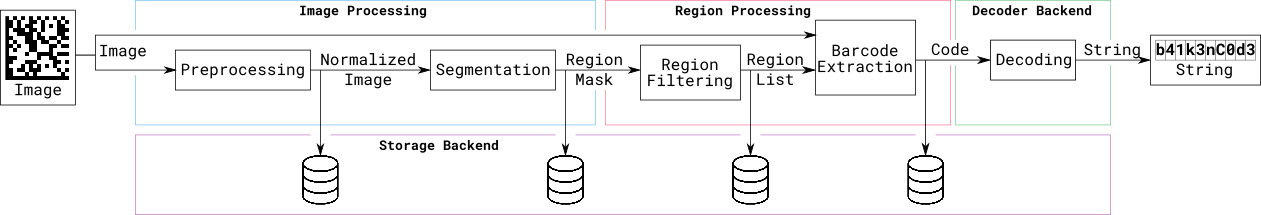
\includegraphics[width=\textwidth]{images/systemdiagram}
  \caption{System diagram}
  \label{fig:systemdiagram}
\end{figure}

A diagram of the modeled system can be seen in Figure~\ref{fig:systemdiagram}.
The system can be split in three mostly independent functional units:
\emph{Image Processing}, \emph{Region Processing} and \emph{Decoding}.
The image processing unit can be modeled around a single concept: the image. 
An image contains a number of points that are arranged in a 2-dimensional space.
Any point in the image is accessible in constant time. Further the image
provides a way to access it's dimensions. An image fulfilling those valid
expressions consequently can be filtered or transformed with every
image processing operation required, most notably, the morphological
operations described in Section~\ref{sec:morph}. After the image segmentation
step, a number of regions of interest (ROIs) are forwarded to the region
processing unit. It's main goal are the filtering of false positives and the
extraction of found barcode regions. The region processing unit operates on
regions and contours. A region represents a set of coherent points in the image. The points
are not required to be in any order. A region allows access to it's
elements and dimensions. Further a regions bounding box and convex hull can be
generated, which are contours. Contours are sets of points that represent a
regions outline when connected in cyclic order. In the final step remaining regions
are extracted from the Image with the help of a minimal bounding box. The decoder unit
then extracts the pure code from the image and decodes it's content.

\section{Implementation}

Considering the adaptability requirement discussed in Section~\ref{sec:requirements}, \emph{balken} is
implemented as a library providing a toolset to efficiently implement a
morphological barcode detection application fitting. Additionally, a detection algorithm
was implemented as a reference. \emph{balken} depends on the \emph{blaze} high
performance math library for it's Matrix types and on the \emph{CImg} library for Image
loading and viewing. Blaze dynamic and static matrix types fulfill the
Image concept and conveniently offer a multitude of performant arithmetic
operations as well as efficient internal memory management and parallelization.

\subsection{Views}

The main considerations in the implementation of the image transformations are the real
time requirement of the application, as well as it's performance. While dynamic
memory allocation is inevitable when dealing with arbitrary sized input images,
it introduces the risk of high latency when requesting memory from the kernel,
which kills every possibility of runtime determinism. It is therefore
favored to use as little dynamic memory as possible.

An elegant solution is the use of views. A view represents a read-only reference
to an object, in this case an Image. Their use lies in the possibility to modify
the way elements of the referred object are accessed. Often views are used to
provide access to a subspace of the elements of the object it refers to.
\emph{balken} uses views to calculate image transformation operations on element
access, and thus drastically reduces the memory usage as resulting values are
generated only when they are read and need not be stored in between processing
steps. The view base class used in balken can be seen in
Listing~\ref{code:viewbase}. 

\begin{lstlisting}[caption=ViewBase, label=code:viewbase]
template <class ImageT, class ViewT>
class ViewBase
{
  using self_t    = ViewBase<ImageT, ViewT>;
  using derived_t = ViewT;

private:
  constexpr const derived_t & derived() const {
    return static_cast<const derived_t &>(*this);
  }

public:
  constexpr ViewBase() = delete;
  constexpr ViewBase(const self_t &) = default;
  constexpr ViewBase(self_t &&) = default;
  constexpr ViewBase(const ImageT & img) : _img{img} {}
  ~ViewBase() = default;

  constexpr decltype(auto) operator()(const size_t i, const size_t j) const {
    return derived().view_element(_img, i, j);
  }

  // Dimensions
  constexpr auto rows() const { return _img.rows(); }
  constexpr auto columns() const { return _img.columns(); }

protected:
  const ImageT & _img;
};
\end{lstlisting}

The classes only member is the image \_img it refers to. The only functions
implemented are the element access function \lstinline{operator()} as well as the
\lstinline{rows()} and \lstinline{columns()} functions, e.G. the basic functions
required to fulfill the image concept requirements discussed in
Section~\ref{sec:concepts}. Listing~\ref{code:binaryview} shows the
implementation of the binary view class, which implements a simple thresholding
transform. The view is initialized with a threshold value. Element access
returns 255 (white) when the value of the referred image lies over the threshold
and 0 (black) when it lies below. The binarize function allows to apply the view
without the explicit need to specify template arguments.

\begin{lstlisting}[caption=BinaryView, label=code:binaryview]
template <class ImageT>
class BinaryView : public view::ViewBase<ImageT, BinaryView<ImageT>>
{
  using self_t = BinaryView<ImageT>;
  using base_t = view::ViewBase<ImageT, self_t>;


public:
  using ElementType = typename ImageT::ElementType;

public:
  constexpr BinaryView(const ImageT & img, const uint8_t threshold)
   : base_t(img), _threshold(threshold) {}


public:
  constexpr ElementType view_element(const ImageT & _img,
                                     std::size_t    i,
                                     std::size_t    j) const {
    return _img(i, j) > _threshold ? 255 : 0;
  }

private:
  const uint8_t _threshold;
};

template <class ImageT>
decltype(auto) binarize(const ImageT & img, std::size_t threshold) {
  return BinaryView<ImageT>(img, threshold);
}
\end{lstlisting}

The binarize function can now be used the same way as an equivalent free
function. It's main advantage is that it does not require additional memory
except for a cheap stack object. As a side effect, the views also prevent
expensive copy operations. In addition the implementation comes with a pipe
operator overload after the model of the \emph{boost.range} library. The goal is
to improve readability of long chains of image transformations. A comparison of
traditional syntax and pipe operator syntax is shown in Listing~\ref{code:pipe}.

\begin{lstlisting}[caption=View Syntax, label=code:pipe]
auto img = load_image(path);

// Traditional syntax
auto traditional = dilate(erode(img, se1) se2);

// Cleaner pipe Syntax
auto pipe = img | dilate(se1) | erode(se2)
\end{lstlisting}


\subsection{Algorithm}

\begin{figure}
  \centering
\begin{subfigure}{.3\textwidth}
  \centering
  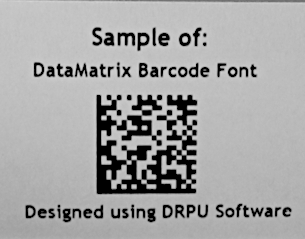
\includegraphics[width=\linewidth]{images/first}
  \caption{Input image}
  \label{fig:sfig1}
\end{subfigure}
\begin{subfigure}{.3\textwidth}
  \centering
  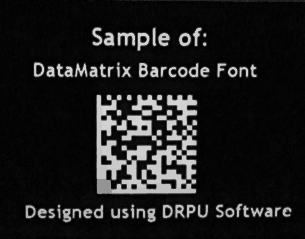
\includegraphics[width=\linewidth]{images/second}
  \caption{Bottom-hat}
  \label{fig:sfig2}
\end{subfigure}
\begin{subfigure}{.3\textwidth}
  \centering
  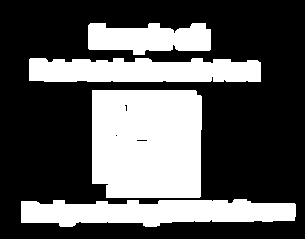
\includegraphics[width=\linewidth]{images/third}
  \caption{Dilation/Erosion}
  \label{fig:sfig2}
\end{subfigure}
\begin{subfigure}{.3\textwidth}
  \centering
  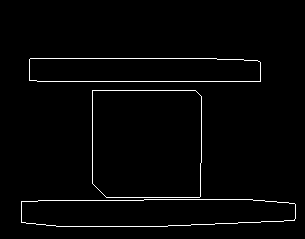
\includegraphics[width=\linewidth]{images/fourth}
  \caption{Regions of Interest}
  \label{fig:sfig2}
\end{subfigure}
\begin{subfigure}{.3\textwidth}
  \centering
  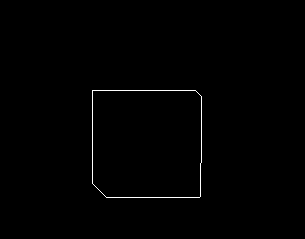
\includegraphics[width=\linewidth]{images/fifth}
  \caption{Filtered regions}
  \label{fig:sfig2}
\end{subfigure}
\caption{Steps of the implemented algorithm}
\label{fig:algo}
\end{figure}

In addition to providing the most important tools to build a morphology based
barcode scanning solution, \emph{balken} implements a reference algorithm
utilizing most of it's build in operations.
The implemented algorithm is based on Katona and Nyúl's works
in~\cite{katona2012novel} and~\cite{katona2013efficient}. The resulting algorithm
is summarized in Algorithm~\ref{alg:detection}. The algorithm receives a
preprocessed image $f$. The preprocessing step consists of a gaussian blur and a
histogram stretch. In the first step a bottom-hat transform is applied to the
image. As described in Section~\ref{sec:morph} the resulting image contains only regions
that were darker than their surroundings in the original image. Due to a high
contrast between the black barcode and it's white surrounding area, the barcode
is extracted cleanly from the original picture. Next the image
is projected into binary space with a threshold value. The image is then dilated
and in the following eroded, which effectively closes down foreground clusters.
The operation is not explicitly noted as a close operation because different
structuring elements may be used for the dilation and erosion.
Finally all clusters are scanned and filter by size and dimensions.
The result of various steps of the algorithm can be seen in Figure~\ref{fig:algo}.

\begin{algorithm}
\caption{Barcode Detection}\label{euclid}
\begin{algorithmic}[1]
\Procedure{FindBarcode}{}
\State $f := (f \bullet SE_1) - f$
\For {all pixels}
\If {$f_{i,j} > i_t$}
\State $f_{i,j} \leftarrow 1$
\Else
\State $f_{i,j} \leftarrow 0$
\EndIf
\EndFor
\State $f := f \oplus SE_2$
\State $f := f \ominus SE_3$
\For {all components}
\If {$ (area > min) \wedge (0.5 < area_{width} / area_{heigth} < 1.5) $}
\State Store component as barcode candidate
\Else
\State Discard component
\EndIf
\EndFor
\EndProcedure
\end{algorithmic}
\label{alg:detection}
\end{algorithm}

\bibliography{literature}
\bibliographystyle{plain}

\end{document}
